\section{Theorie}
\label{sec:Theorie}

\subsection{Kettenschaltungen mit LC-Gliedern}

Kettenschaltungen aus Kondensatoren und Induktivitäten können verschiedene
Frequenzen einer Wechselstromquelle voneinander separieren.
Der sogenannte Tiefpass, der in Abbildung \ref{subfig:Tiefpass}
dargestellt ist, zeichnet
sich dadurch aus, dass er ab einer bestimmten Schwingungsfrequenz die Amplitude
des Wechselstroms verschwinden lässt.
Bei dem sogenannten Hochpass, der in Abbildung \ref{subfig:Hochpass}
abgebildet ist, verschwindet
die Amplitude, wenn die Schwingungsfrequenz gegen Null geht.
Dadurch ist es zum Beispiel möglich die unerwünschten Oberwellen eines
Wechselstromgenerators zu eliminieren, indem ein Tiefpass in die
Schaltung eingebaut wird.

\begin{figure}
  \centering
  \begin{subfigure}{0.48\textwidth}
    \centering
    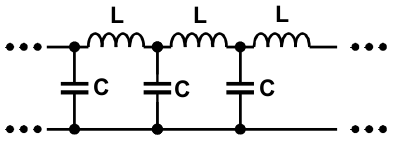
\includegraphics[height=2.5cm]{Tiefpass.png}
    \caption{Tiefpass}
    \label{subfig:Tiefpass}
  \end{subfigure}
  \begin{subfigure}{0.48\textwidth}
    \centering
    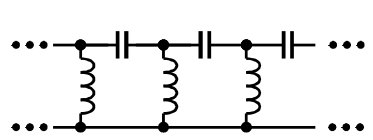
\includegraphics[height=2.5cm]{Hochpass.png}
    \caption{Hochpass}
    \label{subfig:Hochpass}
  \end{subfigure}
  \caption{verschiedene Kettenschaltungen}
  \label{fig:Ketten}
\end{figure}
Im Folgenden werden spezifische Tiefpässe mit konstanten und
alternierenden Kapazitäten analysiert.


\subsection{Dispersionsrelation einer LC-Kettenschaltung}

Über die Kirchhoffschen Gesetze kann mit Hilfe der in Abbildung
\ref{fig:KetteLC} dargestellten Ströme und Spannungen die Schwingungsgleichung
einer LC-Kettenschaltung aufgestellt werden.

\begin{figure}
  \centering
  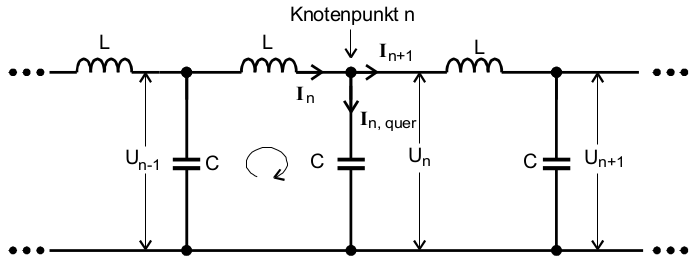
\includegraphics[height=4cm]{KetteLC.png}
  \caption{Ströme und Spannungen in einer LC-Kette}
  \label{fig:KetteLC}
\end{figure}
Aus der Knotenregel

\begin{equation}
  \sum_{n} I_n = 0
  \label{eqn:Knoten}
\end{equation}
folgt

\begin{equation}
  I_n - I_{n+1} - I_{n,\text{quer}} = 0
\end{equation}
und aus der Maschenregel

\begin{equation}
  \sum_{n} U_n = 0
  \label{eqn:Masche}
\end{equation}
im eingeschwungenen Zustand

\begin{equation}
  I_{n} = \frac{U_{n} - U_{n-1}}{\symup{i} \omega L}
\end{equation}
und

\begin{equation}
  I_{n,\text{quer}} = U_{n} \symup{i} \omega C.
\end{equation}
Daraus folgt durch Einsetzen und Umformen die Schwingungsgleichung

\begin{equation}
  \frac{U_{n} - U_{n-1}}{\symup{i} \omega L} - \frac{U_{n+1} - U_{n}}{\symup{i}
  \omega L} - \symup{i} U_{n} \omega C = 0,
\end{equation}
die mit dem Ansatz

\begin{equation}
  U_{n}(t) = U_0 \symup{e}^{\symup{i}t (\omega - n \theta)}
\end{equation}
gelöst werden kann.
Es ergibt sich die Dispersionsrelation

\begin{equation}
  \omega_k(\theta) = \sqrt{\frac{2}{LC}(1-\cos\theta)},
\end{equation}
das ist die Kreisfrequenz
$\omega_k$ in Abhängigkeit von der Phasenverschiebung $\theta$ pro Kettenglied.
Der maximale Wert für $\omega_k$ ist die Grenzfrequenz $\bar{\omega}$
mit

\begin{equation}
  \bar{\omega} = \sqrt{\frac{2}{LC}}.
\end{equation}
Hochfrequentere Schwingungen werden von dem Tiefpass herausgefiltert.


\subsection{Dispersionsrelation einer alternierenden LC-Kettenschaltung}

Mit einer alternierenden LC-Kettenschaltung ist hier ein Tiefpass gemeint,
bei dem zwei unterschiedliche Kapazitäten $C_1$ und $C_2$ alternierend
parallel in die Schaltung eingebaut werden. Dies ist in Abbildung
\ref{fig:KetteLC1C2} dargestellt.

\newpage

\begin{figure}
  \centering
  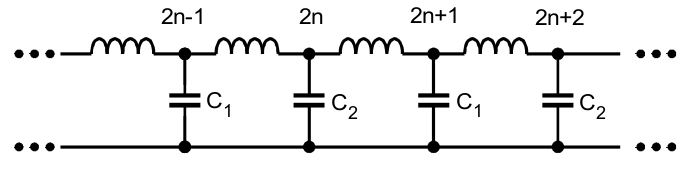
\includegraphics[height=3cm]{KetteLC1C2.png}
  \caption{Knotenpunkte in einer alternierenden LC-Kette}
  \label{fig:KetteLC1C2}
\end{figure}
Aus den Kirchhoffschen Gesetzen \eqref{eqn:Knoten} und \eqref{eqn:Masche}
folgen für diese Schaltung zwei Schwingungsgleichungen

\begin{equation}
  -\omega^2 C_1 U_{2n+1} + \frac{1}{L}(-U_{2n}+2U_{2n+1}-U_{2n+2}) = 0
\end{equation}
und

\begin{equation}
  -\omega^2 C_2 U_{2n} + \frac{1}{L}(-U_{2n+1}+2U_{2n+1}-U_{2n+1}) = 0.
\end{equation}
Durch Einsetzen der Lösungsansätze

\begin{equation}
  U_{2n+1} = U_{0_1} \symup{e}^{\symup{i(\omega t + (2n+1)\theta)}}
\end{equation}
und

\begin{equation}
  U_{2n} = U_{0_2} \symup{e}^{\symup{i(\omega t + 2n\theta)}}
\end{equation}
ergibt sich die Koeffizientenmatrix

\begin{equation}
  \symbf{M} =
  \begin{pmatrix}
    -\omega^2 C_1 + \frac{2}{L} & -\frac{2}{L} \cos \theta \\
    -\frac{2}{L} \cos \theta & -\omega^2 C_2 + \frac{2}{L}
  \end{pmatrix}
  \label{eqn:Matrix}
\end{equation}
mit

\begin{equation}
  \symbf{M} \cdot \vec{U_0} = \vec{0}.
\end{equation}
Um eine nicht-triviale lösung zu erhalten, muss das charakteristische Polyom,
also die Determinante der Matrix \eqref{eqn:Matrix}, Null sein.
Es folgt

\begin{equation}
  \omega^4 - \omega^2 \frac{2}{L} \biggl(\frac{1}{C_1} + \frac{1}{C_2}\biggr)
  \frac{4}{L^2 C_1 C_2} (1 - \cos^2 \theta) = 0
\end{equation}
und daraus zwei sinnvolle Lösungen für die Kreisfrequenz \omega

\begin{equation}
  \omega_1, \omega_2 (\theta) = \sqrt{\frac{1}{L} \biggl(\frac{1}{C_1} +
  \frac{1}{C_2}\biggr)
  \pm \frac{1}{L} \sqrt{\biggl(\frac{1}{C_1} + \frac{1}{C_2}\biggr)^2 -
  \frac{4 \sin^2 \theta}{C_1C_2}}}.
  \label{eqn:Omega}
\end{equation}
Die beiden resultierenden Kurvenäste sind in Abbildung \ref{fig:KurveLC1C2}
dargestellt.

\begin{figure}
  \centering
  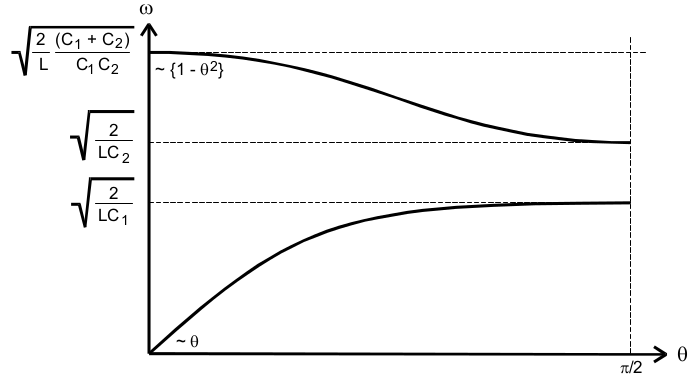
\includegraphics[height=7cm]{KurveLC1C2.png}
  \caption{Skizze der Graphen von $\omega_1$ und $\omega_2$}
  \label{fig:KurveLC1C2}
\end{figure}
Bei dem unteren Kurvenast $\omega_2$ mit negativem Vorzeichen vor der Wurzel
in Gleichung \eqref{eqn:Omega}
steigt die Kreisfrequenz zunächst annähernd konstant an und kann durch die
Gleichung

\begin{equation}
  \omega_2 (\theta) = \sqrt{\frac{2}{L(C_1 + C_2)}} \theta
\end{equation}
beschrieben werden.
Die Funktion erreicht ihren Maximalwert bei $\frac{\pi}{2}$ an
der ersten Grenzfrequenz

\begin{equation}
  \omega_2\Bigl(\frac{\pi}{2}\Bigr) = \bar{\omega}_a = \sqrt{\frac{2}{LC_1}}.
\end{equation}
Bei dem oberen Kurvenast $\omega_1$ mit positivem Vorzeichen vor der Wurzel in
Gleichung \eqref{eqn:Omega} ist die Funktion zunächst annähernd
proportional zu $(1-\theta^2)$.
Sie hat ein Minimum bei der zweiten Grenzfrequenz

\begin{equation}
  \omega_1\Bigl(\frac{\pi}{2}\Bigr) = \bar{\omega}_b = \sqrt{\frac{2}{LC_2}}
\end{equation}
und ein Maximum bei der dritten Grenzfrequenz

\begin{equation}
  \omega_1(0) = \bar{\omega}_c = \sqrt{\frac{2(C_1+C_2)}{LC_1C_2}}.
\end{equation}
Zwischen den Grenzfrequenzen $\bar{\omega}_a$ und $\bar{\omega}_b$ und ab der
oberen Grenzfrequenz $\bar{\omega}_c$ werden alle Frequenzen durch den
Tiefpass herausgefiltert. Die restlichen Frequenzen, die im Wertebereich der
Funktionen $\omega_1$ und $\omega_2$ liegen, werden nicht herausgefiltert.


\subsection{Phasen- und Gruppengeschwindigkeit einer LC-Kettenschaltung}

Die Phasengeschwindigkeit einer Welle ist allgemein die Zeit $t$, die eine
Phasenverschiebung $\theta$ benötigt, um eine bestimmt Strecke zurückzulegen.
In einer Kettenschaltung wird die Strecke durch die Menge an zurückgelegten
Kettengliedern $n$ beschrieben.
Für die allgemeine Phasengeschwindigkeit in der LC-Kette folgt daher

\begin{equation}
  v_\text{ph} = \frac{\Delta n}{\Delta t} = \frac{\omega}{\theta}.
\end{equation}
Bei dieser Phasengeschwindigkeit wurde von einer harmonischen Welle ausgegangen.
Bei einer sogenannten Wellengruppe, die in Abbildung x dargestellt ist,
verhält sich die Phasengeschwindigkeit anders. Nach dem Fourier-Theorem
muss diese Welle frequenzabhängig sein, was zur Folge hat, dass auch die
Phasengeschwindigkeit $v_\text{ph}$ in der LC-Kette von der Frequenz abhängen
muss. Die einzelnen Fourierkomponenten der Welle haben unterschiedliche
Phasengeschwindigkeiten, weshalb die Wellengruppe sich in Zeit und Raum
ausdehnt. Die Ausdehnungsgeschwindigkeit des Wellengruppenmaximums
bezeichnet man als Gruppengeschwindigkeit.


\begin{equation}
1
\end{equation}

Quellen bei Abbildungen !!!


\cite{sample}
